\chapter{Arhitektura i dizajn sustava}
		
		\textbf{\textit{dio 1. revizije}}\\

		\textit{Arhitektura se sastoji od 3 podsustava:}
	\begin{itemize}
		\item 	\textit{Web poslužitelj}
		\item 	\textit{Web aplikacija}
		\item 	\textit{Baza podataka}		
	\end{itemize}
		\textit{
			Web poslužitelj- Primarna zadaća web poslužitelja je komunikacija klijenta s aplikacijom, pomoću HTTP protokola. Web poslužitelj prosljeđuje korisnikov 
			zahtjev, preko Web preglednika, web aplikaciji. 
			Web aplikacija- obrađuje zahtjev te pristupa bazi podataka, vraćajući odgovor korisniku u web pregledniku.
			Baza podataka- implementacija pomoću sql-a.
			Za izradu frontend dijela aplikacije ćemo koristiti Java Script, a za izradu backend dijela aplikacije ćemo koristiti Java Spring Boot. 
			DOVRŠI MVC koncept arhitekture}\\
			
		\section{Baza podataka}
			
			\textbf{\textit{dio 1. revizije}}\\
			Za potrebe našeg sustava koristit ćemo relacijsku bazu podataka koja svojom strukturom olakšava modeliranje stvarnog svijeta. Gradivna jedinka baze je relacija, odnosno tablica koja je definirana svojim imenom i skupom atributa. Zadaća baze podataka je brza i jednostavna pohrana, izmjena i dohvat podataka za daljnju obradu.
			Baza podataka ove aplikacije sastoji se od sljedećih entiteta:
			\begin{itemize}
				\item {Korisnik}
				\item {Doktori-Treneri}
				\item {Recenzije}
				\item {Klijent-Doktor}
				\item {Klijent-Trener}
				\item {KategorijeProizvoda}
				\item {Proizvod}
				\item {NutritivneVrijednosti}
				\item {Vježba}
				\item {Intenzitet}
				\item {BrPotrošenihKalorija}
				\item {Trening}
				\item {NizVježbi}
				\item {Dijeta}
				\item {OgraničenjaNaProizvode}
				\item {OgraničenjaNaKategorije}
				\item {DnevniLimit}
				\item {UneseneNutrVrijednosti}
				\item {KonzumiraniProizvodi}
			\end{itemize}
			
			
		
			\subsection{Opis tablica}
			

				\textbf{Korisnik} Ovaj entitet sadržava sve važne informacije o korisniku aplikacije. Svaki korisnik ima korisničko ime, lozinku, ime, prezime i naziv uloge. 
				
				
				
				\begin{longtabu} to \textwidth {|X[6, l]|X[6, l]|X[20, l]|}
					
					\hline \multicolumn{3}{|c|}{\textbf{Korisnik}}	 \\[3pt] \hline
					\endfirsthead
					
					\hline \multicolumn{3}{|c|}{\textbf{Korisnik}}	 \\[3pt] \hline
					\endhead
					
					\hline 
					\endlastfoot
					
					\cellcolor{LightGreen}korisnickoIme & VARCHAR	&  jedinstveni identifikator korisnika\\ \hline
					Ime	& VARCHAR &  ime korisnika 	\\ \hline 
					Prezime & VARCHAR &  prezime korisnika \\ \hline 
					Lozinka & VARCHAR	& lozinka korisnika 		\\ \hline 
					Uloga	& VARCHAR & Uloga korisnika: doktor, trener ili klijent.  	\\ \hline 
					
					
				\end{longtabu}
				
				\textbf{Doktori-treneri} Da bi neregistrirani korisnik dobio prava doktora i trenera, administrator ga mora potvrditi. Potrebno je dodatno priložiti sliku, email i maksimalni broj korisnika koje želi nadgledati. Navedeni atributi se spremaju u entitet Doktori-Treneri.
				
				
				
				\begin{longtabu} to \textwidth {|X[7, l]|X[6, l]|X[20, l]|}
					
					\hline \multicolumn{3}{|c|}{\textbf{Doktori-Treneri}}	 \\[3pt] \hline
					\endfirsthead
					
					\hline \multicolumn{3}{|c|}{\textbf{Doktori-Treneri}}	 \\[3pt] \hline
					\endhead
					
					\hline 
					\endlastfoot
					
					\cellcolor{LightGreen}korisnickoIme & VARCHAR	&  jedinstveni identifikator korisnika\\ \hline
					E-mail   & VARCHAR &  e-mail adresa doktora/trenera 	\\ \hline 
					Slika  & LONGBLOB &  fotografija doktora/trenera \\ \hline 
					BrojKlijenata& INT	& trenutni broj prijavljenih klijenata 		\\ \hline 
					MaxBrKlijenata	& INT & maksimalan broj prijavljenih klijenata  	\\ \hline 
					
					
				\end{longtabu}
				
				\textbf{Recenzije} Klijent svom doktoru i treneru na profilu može ostaviti recenziju s ocjenom i komentarom, a doktor i trener mogu odgovoriti na vlastitu recenziju. Entitet Recenzije sadrži atribute: korisnickoIme, korImeKlijenta, ocjena, komentar, odgovor i ID komentara. 
				
				\begin{longtabu} to \textwidth {|X[7, l]|X[6, l]|X[20, l]|}
					
					\hline \multicolumn{3}{|c|}{\textbf{Recenzije}}	 \\[3pt] \hline
					\endfirsthead
					
					\hline \multicolumn{3}{|c|}{\textbf{Recenzije}}	 \\[3pt] \hline
					\endhead
					
					\hline 
					\endlastfoot
					\cellcolor{LightGreen} ID & INT & jedinstveni identifikator recenzije \\ \hline
					\cellcolor{LightBlue}korImeKlijenta & VARCHAR	&  jedinstveni identifikator klijenta \\ \hline
					\cellcolor{LightBlue}korisnickoIme   & VARCHAR & jedinstveni identifikator doktora/trenera 	\\ \hline 
					Ocjena  & INT &  ocjena od 1 do 5 \\ \hline 
					Komentar & VARCHAR	& recenzija doktora/trenera 		\\ \hline 
					Odgovor	& VARCHAR & odgovor doktora/trenera na recenziju  	\\ \hline
					
					
					
				\end{longtabu}
				
				\textbf{Klijent-Doktor} Entitet sadrži informacije o trenutnoj suradnji klijenta i nekog doktora. Atributi su: korImeKlijenta i korImeDoktora. 
				
				\begin{longtabu} to \textwidth {|X[7, l]|X[6, l]|X[20, l]|}
					
					\hline \multicolumn{3}{|c|}{\textbf{Klijent-Doktor}}	 \\[3pt] \hline
					\endfirsthead
					
					\hline \multicolumn{3}{|c|}{\textbf{Klijent-Doktor}}	 \\[3pt] \hline
					\endhead
					
					\hline 
					\endlastfoot
					
					\cellcolor{LightGreen}korImeKlijenta & VARCHAR	& jedinstveni identifikator klijenta \\ \hline
					korImeDoktora & VARCHAR & jedinstveni identifikator doktora\\ \hline 
					
				\end{longtabu}
				
				\textbf{Klijent-Trener} Entitet sadrži informacije o trenutnoj suradnji klijenta i nekog trenera. Atributi su: korImeKlijenta i korImeTrenera. 
				
				\begin{longtabu} to \textwidth {|X[7, l]|X[6, l]|X[20, l]|}
					
					\hline \multicolumn{3}{|c|}{\textbf{Klijent-Trener}}	 \\[3pt] \hline
					\endfirsthead
					
					\hline \multicolumn{3}{|c|}{\textbf{Klijent-Trener}}	 \\[3pt] \hline
					\endhead
					
					\hline 
					\endlastfoot
					
					\cellcolor{LightGreen}korImeKlijenta & VARCHAR	&  jedinstveni identifikator klijenta \\ \hline
					korImeTrenera & VARCHAR & jedinstveni identifikator trenera \\ \hline 
					
				\end{longtabu}
				
				\textbf{KategorijeProizvoda} Kategorija proizvoda sadrži više različitih proizvoda sličnih karakteristika, kao što su na primjer tjestenina, proizvodi od mlijeka, meso itd. Entitet KategorijeProizvoda sadrži atribute: ID kategorije i ime kategorije.
				
				\begin{longtabu} to \textwidth {|X[7, l]|X[6, l]|X[20, l]|}
					
					\hline \multicolumn{3}{|c|}{\textbf{KategorijeProizvoda}}	 \\[3pt] \hline
					\endfirsthead
					
					\hline \multicolumn{3}{|c|}{\textbf{KategorijeProizvoda}}	 \\[3pt] \hline
					\endhead
					
					\hline 
					\endlastfoot
					
					\cellcolor{LightGreen}ID & INT	&  jedinstveni identifikator kategorije \\ \hline
					Ime & VARCHAR & ime kategorije 	\\ \hline 
					
				\end{longtabu}
				
				\textbf{Proizvod} Svaki proizvod sadrži sliku, masu i prisutne alergene. Svaki proizvod pripada nekoj kategoriji proizvoda. Entitet Proizvod sadrži atribute: ID proizvoda, masa, slika, prisutni alergeni, ime te ID kategorije.
				
				\begin{longtabu} to \textwidth {|X[7, l]|X[6, l]|X[20, l]|}
					
					\hline \multicolumn{3}{|c|}{\textbf{Proizvod}}	 \\[3pt] \hline
					\endfirsthead
					
					\hline \multicolumn{3}{|c|}{\textbf{Proizvod}}	 \\[3pt] \hline
					\endhead
					
					\hline 
					\endlastfoot
					
					\cellcolor{LightGreen}ID & INT	&  jedinstveni identifikator proizvoda \\ \hline
					Ime & VARCHAR & ime proizvoda 	\\ \hline 
					Masa & DECIMAL & masa proizvoda u gramima\\ \hline
					Slika & LONGBLOB & slika proizvoda\\ \hline
					Alergeni & VARCHAR & popis prisutnih alergena\\ \hline
					\cellcolor{LightBlue}IDkategorije & INT & ID kategorije proizvoda\\ \hline 
					
					
				\end{longtabu}
				
				
				\textbf{NutritivneVrijednosti} Informacije o nutritivnim vrijednostima proizvoda su definirane na 100g, a to su energija, masnoće, zasićene masne kiseline, ugljikohidrati, šećeri, bjelančevine i sol. Entitet NutritivneVrijednosti sadrži istoimene atribute te dodatno ID proizvoda za koji su vrijednosti definirane.  
				
				\begin{longtabu} to \textwidth {|X[8, l]|X[6, l]|X[20, l]|}
					
					\hline \multicolumn{3}{|c|}{\textbf{NutritivneVrijednosti}}	 \\[3pt] \hline
					\endfirsthead
					
					\hline \multicolumn{3}{|c|}{\textbf{NutritivneVrijednosti}}	 \\[3pt] \hline
					\endhead
					
					\hline 
					\endlastfoot
					
					\cellcolor{LightGreen}IDproizvoda & INT	&  jedinstveni identifikator proizvoda \\ \hline
					Energija & DECIMAL & energija u kJ 	\\ \hline 
					Masnoća & DECIMAL & masnoća u sastavu proizvoda\\ \hline
					ZasMasneKiseline & DECIMAL & zasićene masne kiseline u sastavu proizvoda\\ \hline
					Ugljikohidrati & DECIMAL & ugljikohidrati u sastavu proizvoda\\ \hline
					Šećeri & DECIMAL & šećeri u sastavu proizvoda\\ \hline
					Bjelančevine & DECIMAL & bjelančevine u sastavu proizvoda\\ \hline
					Sol & DECIMAL & soli u sastavu proizvoda\\ \hline	
					
					
				\end{longtabu}
				
				\textbf{Vježba} Vježba je definirana sa slikom, opisom i informacijama o broju potrošenih kalorija u sat vremena u ovisnosti o 3 razine intenziteta vježbanja (lagano, normalno, teško). Entitet Vježba dodatno sadrži atribut ID, tj. jedinstveni identifikator vježbe.
				
				\begin{longtabu} to \textwidth {|X[7, l]|X[6, l]|X[20, l]|}
					
					\hline \multicolumn{3}{|c|}{\textbf{Vježba}}	 \\[3pt] \hline
					\endfirsthead
					
					\hline \multicolumn{3}{|c|}{\textbf{Vježba}}	 \\[3pt] \hline
					\endhead
					
					\hline 
					\endlastfoot
					
					\cellcolor{LightGreen}ID & INT	&  jedinstveni identifikator vježbe \\ \hline
					Slika & LONGBLOB & slika vježbe 	\\ \hline 
					Opis & VARCHAR & opis vježbe\\ \hline
					
					
				\end{longtabu}
				\textbf{Intenzitet} Entitet Intenzitet se sastoji od atributa: intenzitet i sifra intenziteta. Intenzitet može biti: lagan, normalan i težak.
				
				\begin{longtabu} to \textwidth {|X[7, l]|X[6, l]|X[20, l]|}
					
					\hline \multicolumn{3}{|c|}{\textbf{Intenzitet}}	 \\[3pt] \hline
					\endfirsthead
					
					\hline \multicolumn{3}{|c|}{\textbf{Intenzitet}}	 \\[3pt] \hline
					\endhead
					
					\hline 
					\endlastfoot
					
					\cellcolor{LightGreen} Šifra & VARCHAR & šifra intenziteta\\ \hline 
					Intenzitet & VARCHAR	&  intenzitet: lagano, normalno ili teško \\ \hline
					
					
				\end{longtabu}
				
				\textbf{BrPotrošenihKalorija} Za svaku vježbu je definiran broj potrošenih kalorija u sat vremena u ovisnosti o 3 razine intenziteta vježbanja (lagano, normalno, teško). 
				
				\begin{longtabu} to \textwidth {|X[8, l]|X[6, l]|X[20, l]|}
					
					\hline \multicolumn{3}{|c|}{\textbf{BrPotrošenihKalorija}}	 \\[3pt] \hline
					\endfirsthead
					
					\hline \multicolumn{3}{|c|}{\textbf{BrPotrošenihKalorija}}	 \\[3pt] \hline
					\endhead
					
					\hline 
					\endlastfoot
					
					\cellcolor{LightGreen}IDvježbe & INT	&  jedinstveni identifikator vježbe \\ \hline
					\cellcolor{LightGreen}šifraIntenziteta & INT & jedinstveni identifikator intenziteta\\ \hline 
					PotrošeneKalorije & DECIMAL & broj potrošenih kalorija u sat vremena
					
					
				\end{longtabu}
				
				
				\textbf{Trening} Trener zadaje trening klijentu svaki dan. Entitet Trening se sastoji od atributa: ID treninga, ID klijenta te datuma.
				
				\begin{longtabu} to \textwidth {|X[7, l]|X[6, l]|X[20, l]|}
					
					\hline \multicolumn{3}{|c|}{\textbf{Trening}}	 \\[3pt] \hline
					\endfirsthead
					
					\hline \multicolumn{3}{|c|}{\textbf{Trening}}	 \\[3pt] \hline
					\endhead
					
					\hline 
					\endlastfoot
					
					\cellcolor{LightGreen}ID & INT	&  jedinstveni identifikator treninga \\ \hline
					IDklijenta & INT & jedinstveni identifikator klijenta\\ \hline 
					Datum & DATETIME & datum treninga\\ \hline
					
					
				\end{longtabu}
				
				\textbf{NizVježbi} Trening se sastoji od niza vježbi koji imaju određeno trajanje i intenzitet. Entitet NizVježbi se sastoji od atributa: ID treninga, ID vježbe, intenzitet vježbe, trajanje vježbe te redni broj vježbe.
				
				\begin{longtabu} to \textwidth {|X[7, l]|X[6, l]|X[20, l]|}
					
					\hline \multicolumn{3}{|c|}{\textbf{NizVježbi}}	 \\[3pt] \hline
					\endfirsthead
					
					\hline \multicolumn{3}{|c|}{\textbf{NizVježbi}}	 \\[3pt] \hline
					\endhead
					
					\hline 
					\endlastfoot
					
					\cellcolor{LightGreen}IDtreninga & INT	&  jedinstveni identifikator treninga \\ \hline
					\cellcolor{LightGreen}RedniBroj & INT & redni broj vježbe\\ \hline
					IDvježbe & INT & jedinstveni identifikator vježbe\\ \hline
					Intenzitet & VARCHAR & intenzitet vježbe (lagano, normalno ili teško)\\ \hline
					Trajanje & INTERVAL & trajanje vježbe\\ \hline
					
					
					
					
				\end{longtabu}
				
				\textbf{Dijeta} Entitet Dijeta se sastoji od atributa: ID dijete, ID klijenta te opisa dijete. Dijetu i potrebne parametre unosi doktor.
				
				\begin{longtabu} to \textwidth {|X[7, l]|X[6, l]|X[20, l]|}
					
					\hline \multicolumn{3}{|c|}{\textbf{Dijeta}}	 \\[3pt] \hline
					\endfirsthead
					
					\hline \multicolumn{3}{|c|}{\textbf{Dijeta}}	 \\[3pt] \hline
					\endhead
					
					\hline 
					\endlastfoot
					
					\cellcolor{LightGreen}ID & INT	&  jedinstveni identifikator dijete \\ \hline
					IDklijenta & INT & jedinstveni identifikator klijenta\\ \hline
					Opis & VARCHAR & opis dijete\\ \hline
					
				\end{longtabu}
				
				\textbf{OgraničenjaNaProizvode} Dijeta se može definirati s ograničenjima na određene proizvode. Entitet Ograničenja se sastoji od atributa: ID dijete i ID proizvoda.
				
				\begin{longtabu} to \textwidth {|X[7, l]|X[6, l]|X[20, l]|}
					
					\hline \multicolumn{3}{|c|}{\textbf{OgraničenjaNaProizvode}}	 \\[3pt] \hline
					\endfirsthead
					
					\hline \multicolumn{3}{|c|}{\textbf{OgraničenjaNaProizvode}}	 \\[3pt] \hline
					\endhead
					
					\hline 
					\endlastfoot
					
					\cellcolor{LightGreen}IDdijete & INT	&  jedinstveni identifikator dijete \\ \hline
					\cellcolor{LightGreen}IDproizvoda & INT & jedinstveni identifikator proizvoda\\ \hline
					
				\end{longtabu}
				
				\textbf{OgraničenjaNaKategorije} Dijeta se može definirati s ograničenjima na određene kategorije proizvoda. Entitet Ograničenja se sastoji od atributa: ID dijete i ID kategorije.
				
				\begin{longtabu} to \textwidth {|X[7, l]|X[6, l]|X[20, l]|}
					
					\hline \multicolumn{3}{|c|}{\textbf{OgraničenjaNaKategorije}}	 \\[3pt] \hline
					\endfirsthead
					
					\hline \multicolumn{3}{|c|}{\textbf{OgraničenjaNaKategorije}}	 \\[3pt] \hline
					\endhead
					
					\hline 
					\endlastfoot
					
					\cellcolor{LightGreen}IDdijete & INT	&  jedinstveni identifikator dijete \\ \hline
					\cellcolor{LightGreen}IDkategorije & INT & jedinstveni identifikator kategorije\\ \hline
					
				\end{longtabu}
				
				\textbf{DnevniLimit} Dijeta se može definirati dnevnim limitom za određene nutritivne vrijednosti proizvoda. Entitet DnevniLimit se sastoji od atributa: ID dijete, limit masnoće, limit ugljikohidrata, limit šećera, limit bjelančevina i limit soli. 
				
				\begin{longtabu} to \textwidth {|X[12, l]|X[6, l]|X[20, l]|}
					
					\hline \multicolumn{3}{|c|}{\textbf{DnevniLimit}}	 \\[3pt] \hline
					\endfirsthead
					
					\hline \multicolumn{3}{|c|}{\textbf{DnevniLimit}}	 \\[3pt] \hline
					\endhead
					
					\hline 
					\endlastfoot
					\cellcolor{LightGreen}IDdijete & INT	&  jedinstveni identifikator dijete \\ \hline
					limitEnergije & DECIMAL & limit energije u kJ 	\\ \hline 
					LimitMasnoće & DECIMAL & limit masnoća u sastavu proizvoda\\ \hline
					LimitZasMasneKiselina & DECIMAL & limit zasićenih masnih kiselina\\ \hline
					LimitUgljikohidrata & DECIMAL & limit ugljikohidrata u sastavu proizvoda\\ \hline
					LimitŠećera & DECIMAL & limit šećera u sastavu proizvoda\\ \hline
					LimitBjelančevina & DECIMAL & limit bjelančevina u sastavu proizvoda\\ \hline
					LimitSoli & DECIMAL & limit soli u sastavu proizvoda\\ \hline	
					
				\end{longtabu}
				
				\textbf{UneseneNutrVrijednosti}  Dijeta se može definirati dnevnim limitom za određene nutritivne vrijednosti proizvoda. Entitet UneseneNutrVrijednosti prati dnevni unos pojedinih nutritivnih vrijednosti. Atributi su: ID korisnika, datum, te unesena energija, masnoće, zasićene masne kiseline, ugljikohidrati, šećeri, bjelančevine i sol.
				
				\begin{longtabu} to \textwidth {|X[8, l]|X[6, l]|X[20, l]|}
					
					\hline \multicolumn{3}{|c|}{\textbf{UneseneNutrVrijednosti}}	 \\[3pt] \hline
					\endfirsthead
					
					\hline \multicolumn{3}{|c|}{\textbf{UneseneNutrVrijednosti}}	 \\[3pt] \hline
					\endhead
					
					\hline 
					\endlastfoot
					\cellcolor{LightGreen} IDklijenta & INT	& jedinstveni identifikator klijenta  \\ \hline
					\cellcolor{LightGreen} Datum & DATETIME	& datum \\ \hline
					Energija & DECIMAL & unesena energija u kJ 	\\ \hline 
					Masnoća & DECIMAL & unesena masnoća\\ \hline
					ZasMasneKiseline & DECIMAL & unesene zasićene masne kiseline\\ \hline
					Ugljikohidrati & DECIMAL & uneseni ugljikohidrati\\ \hline
					Šećeri & DECIMAL & unesena šećeri\\ \hline
					Bjelančevine & DECIMAL & unesene bjelančevine\\ \hline
					Sol & DECIMAL & unesene soli\\ \hline
					
				\end{longtabu}
				
				\textbf{KonzumiraniProizvodi} Entitet KonzumiraniProizvodi se sastoji od atributa: ID klijenta, datum te ID proizvoda. 
				
				\begin{longtabu} to \textwidth {|X[8, l]|X[6, l]|X[20, l]|}
					
					\hline \multicolumn{3}{|c|}{\textbf{KonzumiraniProizvodi}}	 \\[3pt] \hline
					\endfirsthead
					
					\hline \multicolumn{3}{|c|}{\textbf{KonzumiraniProizvodi}}	 \\[3pt] \hline
					\endhead
					
					\hline 
					\endlastfoot
					\cellcolor{LightGreen} IDklijenta & INT	& jedinstveni identifikator klijenta\\ \hline
					\cellcolor{LightGreen} Datum & DATETIME	& datum\\ \hline
					\cellcolor{LightGreen} IDproizvoda & INT & jedinstveni identifikator proizvoda \\ \hline
					
				\end{longtabu}
			
			\subsection{Dijagram baze podataka}
				\textit{ U ovom potpoglavlju potrebno je umetnuti dijagram baze podataka. Primarni i strani ključevi moraju biti označeni, a tablice povezane. Bazu podataka je potrebno normalizirati. Podsjetite se kolegija "Baze podataka".}
			
			\eject
			
			
		\section{Dijagram razreda}
		
			\textit{Potrebno je priložiti dijagram razreda s pripadajućim opisom. Zbog preglednosti je moguće dijagram razlomiti na više njih, ali moraju biti grupirani prema sličnim razinama apstrakcije i srodnim funkcionalnostima.}\\
			
			\textbf{\textit{dio 1. revizije}}\\
			
			\begin{figure}[H]
			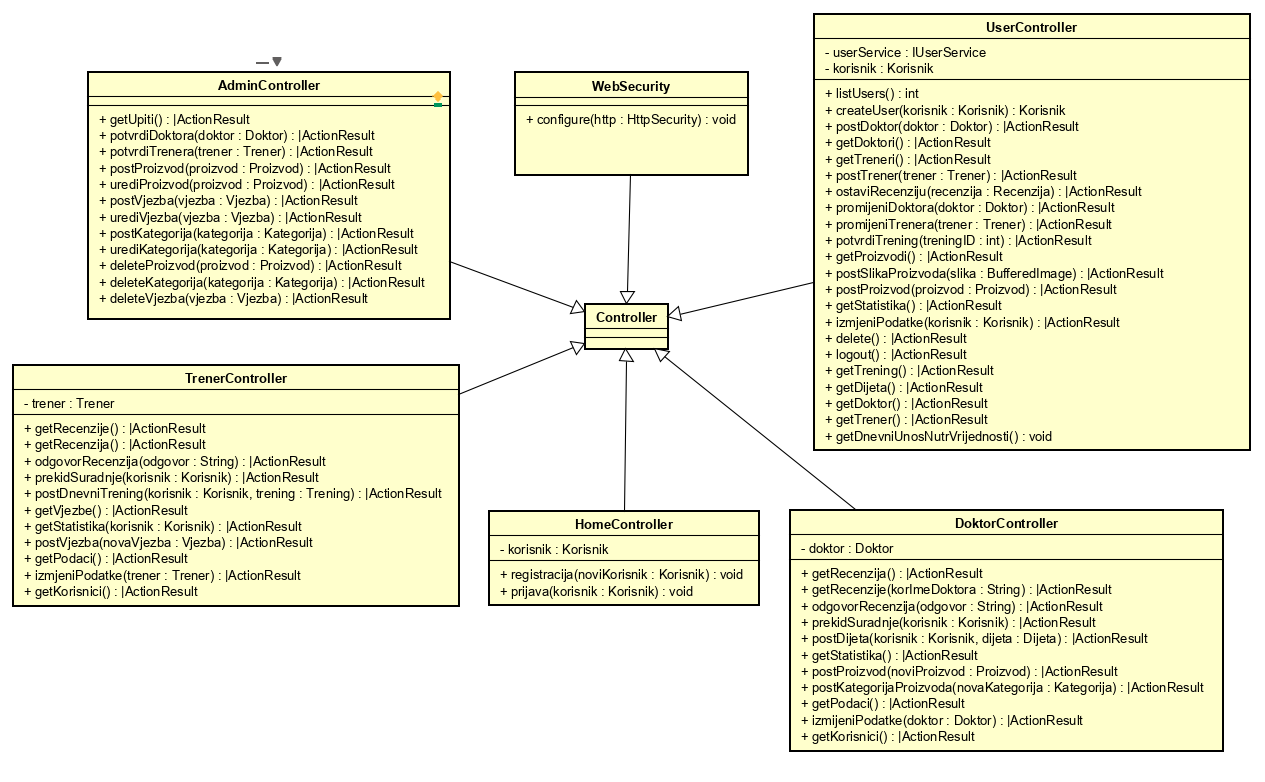
\includegraphics[scale=0.65]{slike/Controlleri.PNG}
			\centering
			\caption{Dijagram razreda - dio Controlleri}
			\label{fig:promjene}
			\end{figure}

			\begin{figure}[H]
			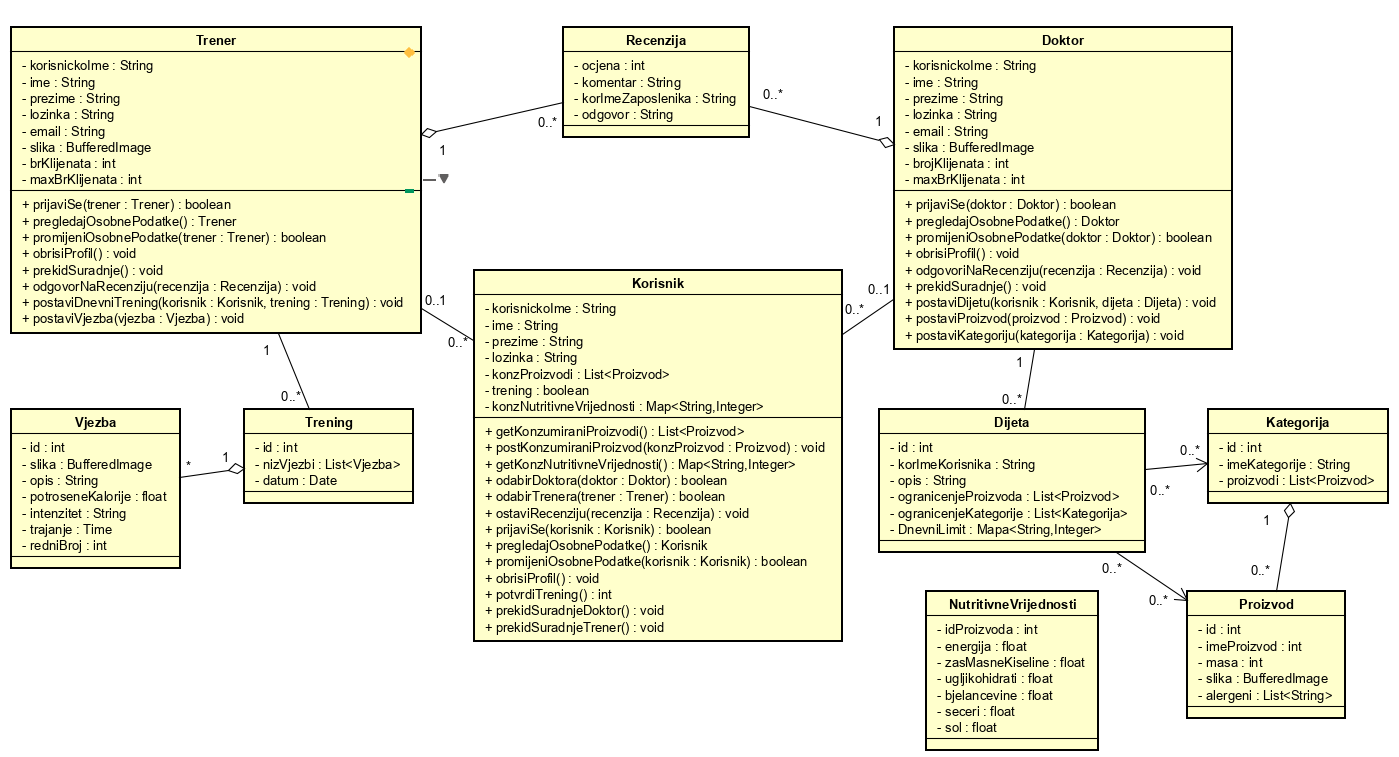
\includegraphics[scale=0.6]{slike/Modeli.PNG}
			\centering
			\caption{Dijagram razreda - dio Modeli}
			\label{fig:promjene}
			\end{figure}
			
			\textbf{\textit{dio 2. revizije}}\\			
			
			\textit{Prilikom druge predaje projekta dijagram razreda i opisi moraju odgovarati stvarnom stanju implementacije}
			
			
			
			\eject
		
		\section{Dijagram stanja}
			
			
			\textbf{\textit{dio 2. revizije}}\\
			
			\textit{Potrebno je priložiti dijagram stanja i opisati ga. Dovoljan je jedan dijagram stanja koji prikazuje \textbf{značajan dio funkcionalnosti} sustava. Na primjer, stanja korisničkog sučelja i tijek korištenja neke ključne funkcionalnosti jesu značajan dio sustava, a registracija i prijava nisu. }
			
			
			\eject 
		
		\section{Dijagram aktivnosti}
			
			\textbf{\textit{dio 2. revizije}}\\
			
			 \textit{Potrebno je priložiti dijagram aktivnosti s pripadajućim opisom. Dijagram aktivnosti treba prikazivati značajan dio sustava.}
			
			\eject
		\section{Dijagram komponenti}
		
			\textbf{\textit{dio 2. revizije}}\\
		
			 \textit{Potrebno je priložiti dijagram komponenti s pripadajućim opisom. Dijagram komponenti treba prikazivati strukturu cijele aplikacije.}